% GNUPLOT: LaTeX picture with Postscript
\begingroup
  \makeatletter
  \providecommand\color[2][]{%
    \GenericError{(gnuplot) \space\space\space\@spaces}{%
      Package color not loaded in conjunction with
      terminal option `colourtext'%
    }{See the gnuplot documentation for explanation.%
    }{Either use 'blacktext' in gnuplot or load the package
      color.sty in LaTeX.}%
    \renewcommand\color[2][]{}%
  }%
  \providecommand\includegraphics[2][]{%
    \GenericError{(gnuplot) \space\space\space\@spaces}{%
      Package graphicx or graphics not loaded%
    }{See the gnuplot documentation for explanation.%
    }{The gnuplot epslatex terminal needs graphicx.sty or graphics.sty.}%
    \renewcommand\includegraphics[2][]{}%
  }%
  \providecommand\rotatebox[2]{#2}%
  \@ifundefined{ifGPcolor}{%
    \newif\ifGPcolor
    \GPcolortrue
  }{}%
  \@ifundefined{ifGPblacktext}{%
    \newif\ifGPblacktext
    \GPblacktexttrue
  }{}%
  % define a \g@addto@macro without @ in the name:
  \let\gplgaddtomacro\g@addto@macro
  % define empty templates for all commands taking text:
  \gdef\gplbacktext{}%
  \gdef\gplfronttext{}%
  \makeatother
  \ifGPblacktext
    % no textcolor at all
    \def\colorrgb#1{}%
    \def\colorgray#1{}%
  \else
    % gray or color?
    \ifGPcolor
      \def\colorrgb#1{\color[rgb]{#1}}%
      \def\colorgray#1{\color[gray]{#1}}%
      \expandafter\def\csname LTw\endcsname{\color{white}}%
      \expandafter\def\csname LTb\endcsname{\color{black}}%
      \expandafter\def\csname LTa\endcsname{\color{black}}%
      \expandafter\def\csname LT0\endcsname{\color[rgb]{1,0,0}}%
      \expandafter\def\csname LT1\endcsname{\color[rgb]{0,1,0}}%
      \expandafter\def\csname LT2\endcsname{\color[rgb]{0,0,1}}%
      \expandafter\def\csname LT3\endcsname{\color[rgb]{1,0,1}}%
      \expandafter\def\csname LT4\endcsname{\color[rgb]{0,1,1}}%
      \expandafter\def\csname LT5\endcsname{\color[rgb]{1,1,0}}%
      \expandafter\def\csname LT6\endcsname{\color[rgb]{0,0,0}}%
      \expandafter\def\csname LT7\endcsname{\color[rgb]{1,0.3,0}}%
      \expandafter\def\csname LT8\endcsname{\color[rgb]{0.5,0.5,0.5}}%
    \else
      % gray
      \def\colorrgb#1{\color{black}}%
      \def\colorgray#1{\color[gray]{#1}}%
      \expandafter\def\csname LTw\endcsname{\color{white}}%
      \expandafter\def\csname LTb\endcsname{\color{black}}%
      \expandafter\def\csname LTa\endcsname{\color{black}}%
      \expandafter\def\csname LT0\endcsname{\color{black}}%
      \expandafter\def\csname LT1\endcsname{\color{black}}%
      \expandafter\def\csname LT2\endcsname{\color{black}}%
      \expandafter\def\csname LT3\endcsname{\color{black}}%
      \expandafter\def\csname LT4\endcsname{\color{black}}%
      \expandafter\def\csname LT5\endcsname{\color{black}}%
      \expandafter\def\csname LT6\endcsname{\color{black}}%
      \expandafter\def\csname LT7\endcsname{\color{black}}%
      \expandafter\def\csname LT8\endcsname{\color{black}}%
    \fi
  \fi
  \setlength{\unitlength}{0.0500bp}%
  \begin{picture}(7200.00,5040.00)%
    \gplgaddtomacro\gplbacktext{%
      \csname LTb\endcsname%
      \put(1122,704){\makebox(0,0)[r]{\strut{}$0.5$}}%
      \put(1122,1156){\makebox(0,0)[r]{\strut{}$1$}}%
      \put(1122,1609){\makebox(0,0)[r]{\strut{}$1.5$}}%
      \put(1122,2061){\makebox(0,0)[r]{\strut{}$2$}}%
      \put(1122,2514){\makebox(0,0)[r]{\strut{}$2.5$}}%
      \put(1122,2966){\makebox(0,0)[r]{\strut{}$3$}}%
      \put(1122,3419){\makebox(0,0)[r]{\strut{}$3.5$}}%
      \put(1122,3871){\makebox(0,0)[r]{\strut{}$4$}}%
      \put(1122,4324){\makebox(0,0)[r]{\strut{}$4.5$}}%
      \put(1122,4776){\makebox(0,0)[r]{\strut{}$5$}}%
      \put(1254,484){\makebox(0,0){\strut{}$0.00040$}}%
      \put(2190,484){\makebox(0,0){\strut{}$0.00060$}}%
      \put(3126,484){\makebox(0,0){\strut{}$0.00080$}}%
      \put(4062,484){\makebox(0,0){\strut{}$0.00100$}}%
      \put(4998,484){\makebox(0,0){\strut{}$0.00120$}}%
      \put(5934,484){\makebox(0,0){\strut{}$0.00140$}}%
      \put(6870,484){\makebox(0,0){\strut{}$0.00160$}}%
      \put(484,2740){\rotatebox{90}{\makebox(0,0){\strut{}$\beta$}}}%
      \put(4062,154){\makebox(0,0){\strut{}$\bar{S}$}}%
    }%
    \gplgaddtomacro\gplfronttext{%
      \csname LTb\endcsname%
      \put(5883,4603){\makebox(0,0)[r]{\strut{}Section B FORM}}%
      \csname LTb\endcsname%
      \put(5883,4383){\makebox(0,0)[r]{\strut{}Section B Monte Carlo}}%
    }%
    \gplbacktext
    \put(0,0){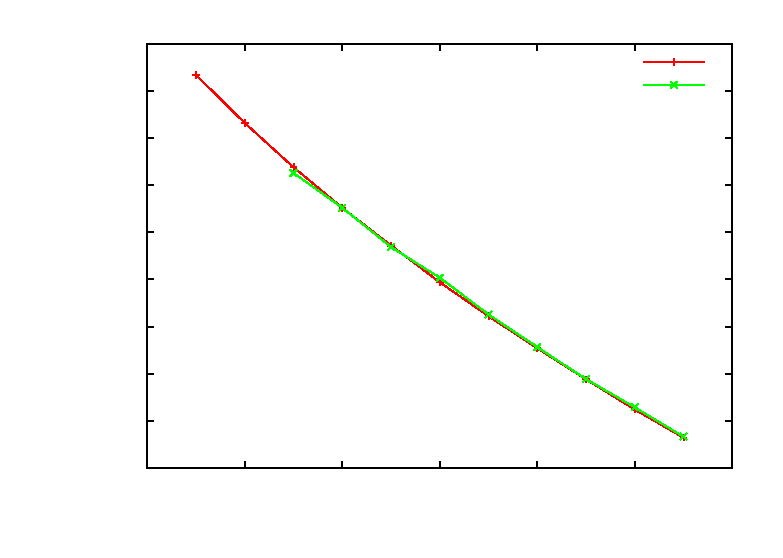
\includegraphics{verification_s}}%
    \gplfronttext
  \end{picture}%
\endgroup
